Nesta seção é apresentado em detalhes a implementação aplicadas no \textit{benchmark} Bench4Q. A Figura \ref{fig:diagrama-classes} mostra o diagrama de classes envolvido na extensão do Bench4Q. As classes sinalizadas na core azul, representa as já existentes mas que passaram por adaptações e modificações, ja as classes na cor verde, se refere as novas classes criadas para possibilitar a modelagem da carga no Bench4Q.

\begin{figure}[htb]
	\centering
	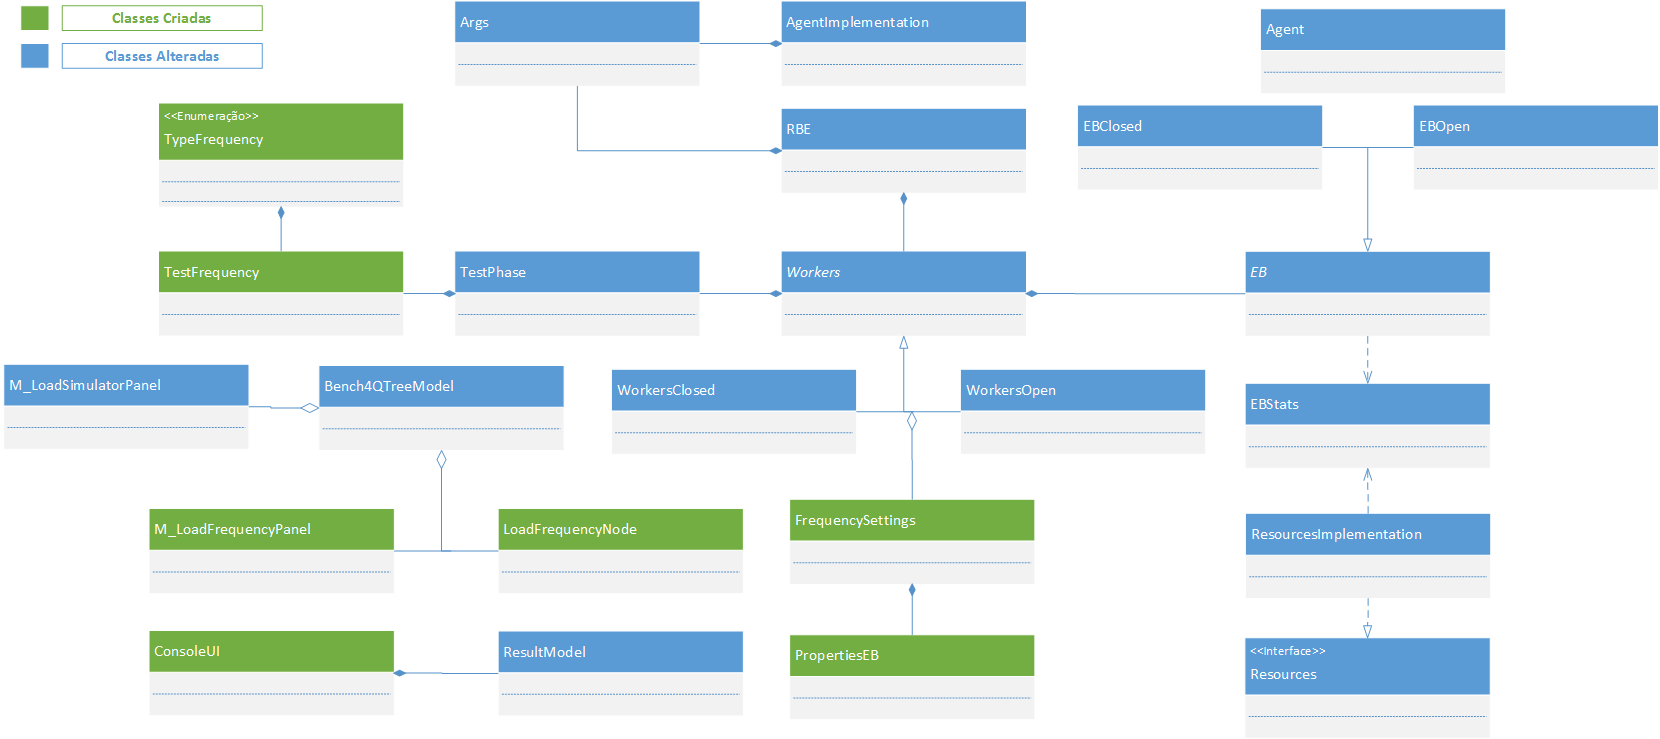
\includegraphics[scale=0.4]{diagrama-classes-beanch4Q.png}	
	\caption{Diagrama de classes da extensão do Bench4Q.}
	\label{fig:diagrama-classes}
	\fautor
\end{figure}

%1º  - falar como foi implementados as modificações conforme a metodologia

A principio foi identificado o modulo de geração de carga do Bench4Q e este passou por alterações para gerar a carga de trabalho esperada. Conforme o diagrama de classes na figura \ref{fig:diagrama-classes}, é possível ter uma ideia do trabalho realizado no \textit{benchmark}, vale aqui salientar que o Bench4Q é uma ferramente completa e extensa, e diagramar todas as classes do mesmo ficaria difícil a sua apresentação em um único diagrama que facilita-se o entendimento, sendo assim, aqui apresentamos somente as classes já existente no Bench4Q e que passar por modificações para atender aos requisitos da metodologia e as novas classes que foram necessária para o mesmo objetivo.
O Bench4Q fornece uma estrutura e componentes compartilhados para a comunicação entre os dois principais módulos da carga de trabalho, \textbf{Console} e \textbf{Agente}. A extensão é construído em sob a classe \textsf{MLoadSimulatorPanel}, que orquestra toda a interatividade gráfica do Bench4Q. O novo painel de configuração, que modula a carga, \textsf{MLoadFrequencyPanel} estende da classe original \textsf{Bench4QTreeModel} adicionando os parâmetros para a modulação: tipo da carga, o instante em que a carga se inicia, o tempo de atuação da carga e a quantidade de EBs que atuaram nessa carga, esses parâmetros são armazenados na classe \textsf{TestFrequency} que são repassadas para a classe \textsf{PropertiesEB} através da \textsf{FrequencySettings}. Nas classes \textsf{Agent}, \textsf{EB}, \textsf{EBClose}, \textsf{EBOpen}, \textsf{Workers}, \textsf{WorkersClosed} e \textsf{WorkersOpen} foram modificadas para receber os novos parâmetros da \textsf{TestFrequency} e compreendê-los correspondentemente a modulação configurada e gerando a carga durante a execução.

Este conjunto de classes é que lida, manipula e gerencia a carga de trabalha gerada pelo Beanch4Q. A ferramente utiliza de um excelente console para configurar a carga de trabalho, e para mantar e respeitar o padrão do \textit{benchmark} foi implementado uma interface de configuração conforme ilustrado na figura \ref{fig:interface-criada-beanch4q}. Seguindo os padrões do Bench4Q, foi criado uma interface por onde controlar o comportamento da carga antes da execução, a carga é programada atras vezes de parâmetros informados previamente a execução do experimento. Exemplo, ao escolher a opção degrau, é necessário informar quantos EBs geram o degrau, em que instante de tempo, e qual o tempo de duração e por fim qual a sua polaridade (com base em um pulso elétrico a positiva sairia de zero e chega a um, a negativa, sairia de um e chegaria a zero).

\begin{figure}[htb]
	\centering
	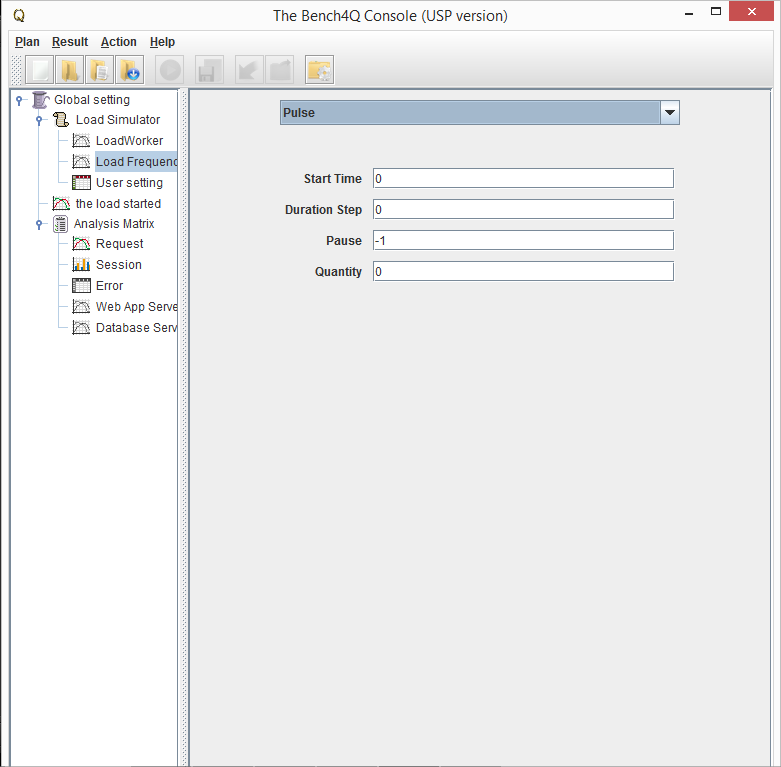
\includegraphics[scale=0.5]{console-bench4Q-usp.png}
	\caption{Console de programação de carga de trabalho.}
	\label{fig:interface-criada-beanch4q}
	\fautor
\end{figure}


%- mostrar resultados da carga de trabalho

%2º  - falar que nao foram necessarios incluir novas metricas, pois as presentes no bench4 já são o suficiente para o estudo de caso

%Para iniciar o desenvolvimento de extensão do Bench4Q, iniciamos por trabalhar com uma versão completa da implementação do \textit{benchmark} Bench4Q \textbf{(adicionar link de download da ferramenta)}

%Considere uma livraria que desejar realizar uma promoção no dia de seu aniversario, essa promoção é ousada e espera-se ter um grande volume de vendas decorre a comemoração, isso irá apoiar as suas operações de venda e expandir seu mercado. Logo, a maior preocupação por parte da empresa é que seu \textit{e-commerce} esteja disponível para os compradores/clientes, assim a empresa decidiu contratar os serviços de uma provedora de \textit{Cloud Computing} para hospedar o seu \textit{e-commerce} no dia o evento. O ambiente destinado para este evento está em processo de validação de carga, por parte da operadora, para garantir que os clientes antigos e novos da livraria possam usufruir e aproveitarem a promoção, e para a provedora não correr o risco de perderem o contrato o diretor de TI da provedora solicitou a sua equipe de engenheiros realizarem experimentos para garantir o desempenho esperado pelo cliente contrante.
%Supondo que, em condições normais de funcionamento, o \textit{e-commerce} da livraria tem 10 clientes simultâneos e durante o dia do evento da mega promoção de aniversario, espera-se em média 20 clientes simultâneos,  além disso, a carga de trabalho está prevista para crescer em até 300\% ao longo do dia. A empresa contrante, a livraria, acredita que o tempo médio de resposta para todas as operações é de 7 segundos, e deseja que 90\% dos seus clientes estejam dentro dessas condições pré estabelecidas por ela, ou seja, a livraria da um margem de 10\% dos cliente fiquem fora do desempenho definido. Note-se que todos estes números e valores foram escolhidos de forma arbitrária, de modo a tornar o nosso cenário motivador mais específico.
%Ao ler os requisitos de desempenho, a equipe de engenheiros, vez a necessidade de uma analise transiente, que por sua vez, buscam um \textit{becnhmark} para realizar os experimentos, então identificam um \textit{becnhmark} que se adéqua-se ao caso, entretanto o \textit{becnhmark} em questão não realiza analise transiente, contudo a equipe decide em aplicar a metodologia proposta neste trabalho.

%Ainda assim, a equipe de engenheiro da operadora de \textit{Cloud Computing} precisa garantir e encontrar respostas para as seguintes perguntas, após a aplicação da metodologia:

%\begin{itemize}
%	\item Com a aplicação da metodologia, o \textit{becnhmark} irá estimular o sistema a apresentar a sua dinâmica, permitindo a analise em regime transiente do mesmo? 
%	\item Que as métricas utilizadas pelo contratante são sendo analisadas
%\end{itemize}





